%%%%%%%%%%%%%%%%%%%%%%%%%%%%%%%%%%%%%%%%%%%%%%%%%%%%%%%%%%%%%%%%%%%%%%
% How to use writeLaTeX: 
%
% You edit the source code here on the left, and the preview on the
% right shows you the result within a few seconds.
%
% Bookmark this page and share the URL with your co-authors. They can
% edit at the same time!
%
% You can upload figures, bibliographies, custom classes and
% styles using the files menu.
%
%%%%%%%%%%%%%%%%%%%%%%%%%%%%%%%%%%%%%%%%%%%%%%%%%%%%%%%%%%%%%%%%%%%%%%

\documentclass[12pt]{article}
\usepackage{sbc-template}
\usepackage{graphicx,url}
%\usepackage[brazil]{babel}   
\usepackage[utf8]{inputenc}  
\usepackage{float}

\sloppy
\title{Análise de Desempenho de Algoritmos Clássicos de Ordenação}
\author{Daniel Matos Marques}
\address{Instituto de Ciências Exatas \\ Pontifícia Universidade Católica de Minas Gerais (PUC-MG)}

\begin{document} 

\maketitle

\begin{resumo}
Este trabalho apresenta uma análise comparativa entre quatro algoritmos clássicos de ordenação: Selection Sort, Insertion Sort, Bubble Sort e Quicksort. Os algoritmos foram implementados em Java e avaliados quanto ao tempo de execução, número de comparações e movimentações realizadas em vetores de inteiros aleatórios com tamanhos de 100, 1000, 10000 e 100000 elementos. Os resultados são apresentados graficamente e discutidos criticamente, com destaque para a eficiência de cada algoritmo conforme o aumento da entrada.
\end{resumo}

\section{Introdução}

Algoritmos de ordenação são fundamentais na computação, sendo amplamente utilizados em diversas aplicações. Este trabalho visa comparar algoritmos clássicos quanto ao desempenho prático em três aspectos principais: tempo de execução, número de comparações e movimentações de elementos.

\section{Metodologia}

Foram implementados os algoritmos de ordenação Selection Sort, Insertion Sort, Bubble Sort e Quicksort em Java. Cada algoritmo foi executado sobre vetores gerados aleatoriamente com tamanhos de 100, 1000, 10000 e 100000 elementos. Para cada execução, registrou-se:
\begin{itemize}
  \item Tempo de execução (em milissegundos)
  \item Número de comparações
  \item Número de movimentações (trocas)
\end{itemize}

\newpage

\section{Resultados}

\subsection{Tempo de Execução}
\begin{figure}[H]
\centering
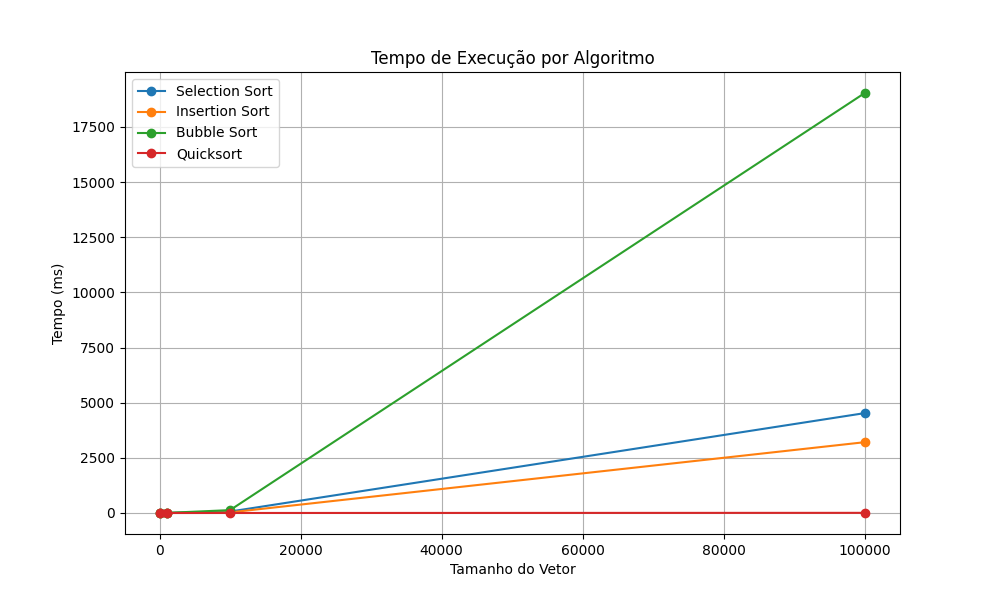
\includegraphics[width=.5\textwidth]{tempo.png}
\caption{Tempo de execução por algoritmo e tamanho de entrada}
\end{figure}

\subsection{Comparações}
\begin{figure}[H]
\centering
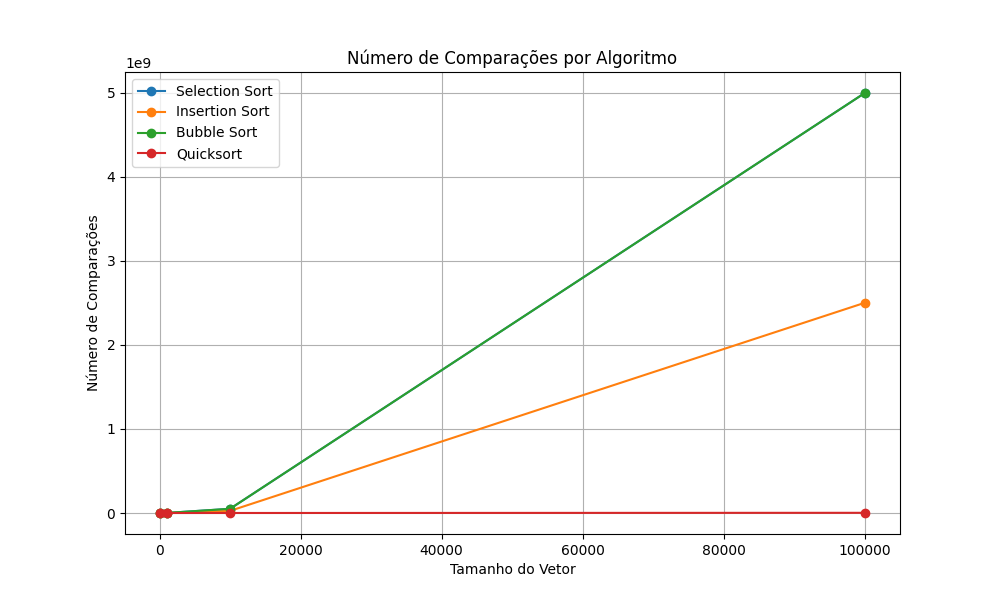
\includegraphics[width=.5\textwidth]{comparacoes.png}
\caption{Número de comparações realizadas por cada algoritmo}
\end{figure}

\subsection{Movimentaçõees}
\begin{figure}[H]
\centering
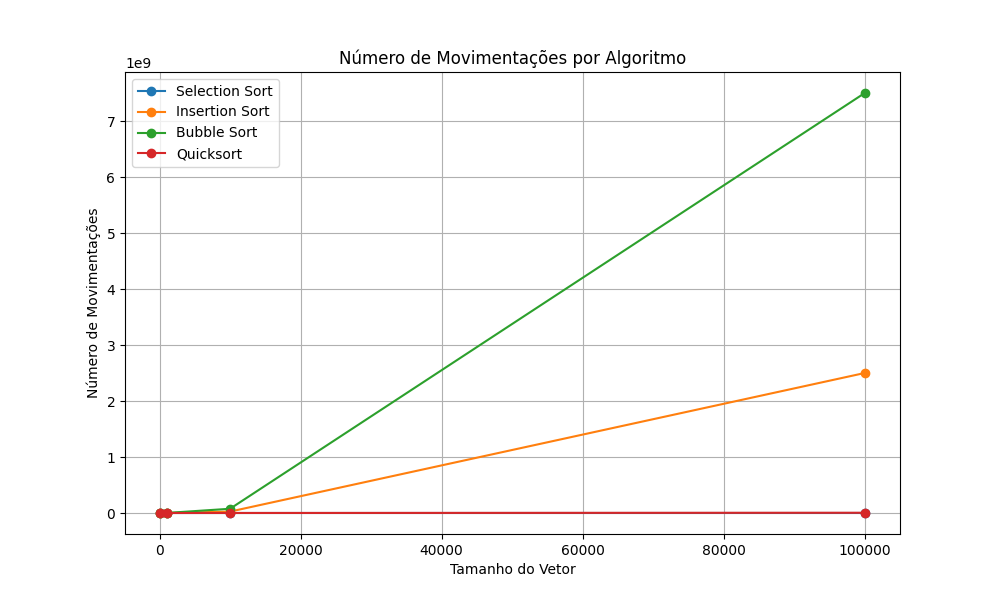
\includegraphics[width=.5\textwidth]{movimentacoes.png}
\caption{Número de movimentações realizadas por cada algoritmo}
\end{figure}

\newpage

\section{Análise Crítica}

Os algoritmos de ordenação simples (Selection, Insertion e Bubble) demonstraram desempenho pobre para entradas grandes, com tempos de execução e número de operações crescendo rapidamente. O Quicksort, por outro lado, manteve desempenho superior mesmo em entradas com 100000 elementos.

Em termos de comparações, o Quicksort foi o mais eficiente, seguido pelo Insertion Sort para entradas menores. O Selection Sort, apesar de realizar menos movimentações, faz muitas comparações.

\section{Conclusão}

A análise evidencia que algoritmos de ordenação simples são adequados apenas para conjuntos pequenos. O Quicksort destacou-se como a melhor escolha para entradas maiores, sendo mais eficiente tanto em tempo quanto em operações. Esta comparação reforça a importância de escolher algoritmos adequados ao contexto e ao volume de dados.

\end{document}
